\documentclass[12pt]{article}
\usepackage[a4paper, total={6in, 9in}]{geometry}
\usepackage{graphicx} % Required for inserting images
\usepackage{blindtext}
\usepackage[T1]{fontenc}
\usepackage{hyperref}
\usepackage[sorting = none]{biblatex}
\usepackage{setspace}
\usepackage{listings}
\usepackage{bm}
\usepackage{amsmath}
\usepackage{amsfonts}
\usepackage{mathtools}
\usepackage{algorithm}
\usepackage{algpseudocode}
\usepackage{tabularx} \newcolumntype{Y}{>{\centering\arraybackslash}X}

\addbibresource{bibliography.bib}
\hypersetup{
    colorlinks=true,
    citecolor=black,
    filecolor=black,
    linkcolor=black,
    urlcolor=black
}

\newcommand{\bx}{\bm x}

\newcommand{\map}{\xlongrightarrow{\text{M}}}
\newcommand{\reduce}{\xlongrightarrow{\text{R}}}

\algnewcommand\algorithmicforeach{\textbf{for each}}
\algdef{S}[FOR]{ForEach}[1]{\algorithmicforeach\ #1\ \algorithmicdo}

\algblock{Input}{EndInput}
\algnotext{EndInput}
\algblock{Output}{EndOutput}
\algnotext{EndOutput}
\newcommand{\Desc}[2]{\State \makebox[2em][l]{#1}#2}

% ----------------------------------------------------------

\title{AMD-SMML Joint Project\\
\large Analysis of ``IBM Transactions for Anti Money Laundering'' dataset}
\author{Federico Bruzzone, Ivan Mazzon}
\date{October 2023}

\begin{document}

\vspace*{\fill}
\begin{minipage}{0.9\textwidth}
\maketitle
\end{minipage}
\vspace*{\fill}

{
\footnotesize
Github repository: \url{https://github.com/FedericoBruzzone/anti-money-laundering/}
}

\vspace{1cm}

\fbox{
    \begin{minipage}{0.9\textwidth}
    \footnotesize\itshape
    We declare that this material, which we now submit for assessment, is entirely our own work and has not been taken from the work of others, save and to the extent that such work has been cited and acknowledged within the text of our work. We understand that plagiarism, collusion, and copying are grave and serious offences in the university and accept the penalties that would be imposed should we engage in plagiarism, collusion or copying. This assignment, or any part of it, has not been previously submitted by us or any other person for assessment on this or any other course of study.
    \end{minipage}
}

\thispagestyle{empty}

\newpage
\thispagestyle{empty}
\setcounter{page}{0}

\onehalfspace
{
\tableofcontents
}

\newpage

\section{Introduction}

The money laundering detection is a considerable problem in machine learning.
The difficulty of this problem is due to high imbalanced available data, in detail the shortage of examples of illegal operations, that we will call ``positive'' instances.
In this project we have provided an implementation of three tree learning algorithm for binary classification to face this problem: ID3 \cite{ID3}, C4.5 \cite{C4.5} and a custom algorithm inspired by techniques used in ID3.
Each algorithm is also used to induce a random forest using the Spark framework \cite{SparkUrl}.



\section{Preliminary Dataset Analysis}

``IBM Transactions for Anti Money Laundering'' provides several dataset each of which consists in transactions data.

In every dataset, the value of every attribute is known, then, we will assume that every observation given to the model, in both fitting and training processes, will be complete.
% during the construction of trees, the handling of missing values won't be necessary.
Nevertheless, a handling method for unseen values in training phase will be required. Since the training set will be extract randomly from a whole dataset, it could happen that each attribute does not take all possible unique values and in the test set there might be unseen values.

Every dataset of the repository is affected by unbalanced labeling. It means that instances that belong to positive class are very infrequent.
It has observed in literature that unbalanced labeling induce a proclivity in traditional learning models to learn more from examples belonging to the majority class and consequently most of new instances will be classified with that class \cite{Ling2010, ClassImbalanceProblem}.
Some provided datasets have a higher illicit ratio, but it's not enough because the ratio between number of positive and negative is however very low.
For example, that ratio in \texttt{HI-Small\_Trans} dataset is $5 \cdot 10^{-4}$.

To cope with high unbalanced labeling of examples in the training set, we have chosen to evaluate some preprocessing techniques to mitigate the problem and confidently obtain higher performance of classification. They are the following:
%
\begin{itemize}
    \setlength\itemsep{0cm}
    \item undersampling: it consists in discarding random examples of majority class in order to balance the training set.
    \item oversampling: it consists in adding multiple copies of every example of minority class in the training set.
\end{itemize}
%
% Another method that can be adopted is the cost sensitive learning.\\
% (......)

It can be noticed that the dataset contains several categorical attributes. Generally, during the fitting procedure of a machine learning model, many comparisons between values of attributes are needed. Since equality checking between integers is more efficient than between strings, we have implemented an encoding system to convert values of attributes from strings to integers to obtain a homogeneous type representation.

The datasets have an attribute \texttt{Timestamp} which can be split in three attributes \texttt{Date}, \texttt{Hour} and \texttt{Minute}, trying to generate more useful data to process.

\newpage
\section{Implemented Algorithms}
In this section we explain the algorithms we have implemented.
To this aim, we introduce the following notation.
Let $T$ the considered training set.
The instances in $T$ are in the form $(\bx, y)$, where $\bx=(x_1, \dots, x_n)$ is the vector of $n$ values of $X_1, \dots, X_n$ attributes and $y \in \{0,1\}$ is the classification given a priori, since we are operating in a binary classification context.
Let $N_c(S)$ the number of class $c \in C = \{c^+, c^-\}$ instances over set $S$.
% Let the classes be $\{C^-, C^+\}$, respectively negative and positive.

\subsection{ID3}
Introduced by J.R. Quinlan in 1986, ID3 \cite{ID3} is an algorithm that induces tree predictors adopting a greedy divide-et-impera strategy. In detail, when a node is considered, starting by the root, the algorithm selects the best split option at the moment and subdivides the problem in smaller ones.

\paragraph{The information gain criterion.} ID3 uses an index called \emph{information gain} as split quality indicator.
%
The information gain of an attribute $X$ over a set of instances $T$ is calculated in the following way:
\begin{equation}  \label{eq:id3_infogain}
    gain(X) = info(T) - info_X(T)
\end{equation}
where
\begin{equation} \label{eq:id3_info}
    info(T) = - \sum_{c \in C} \frac{N_c(T)}{|T|} \cdot \log_2 \frac{N_c(T)}{|T|}
\end{equation}
is the entropy function and, being $T_1, \dots, T_s$ the partitions of $T$ consisting of instances grouped by the value of the attribute $X$ ($s$ distinct values),
\begin{equation} \label{eq:id3_info_X}
    info_X(T)= \sum_{i=1}^s \frac{|T_i|}{|T|} \cdot info(T_i) \;.
\end{equation}
The gain criterion selects the attribute that maximize the information gain.

\newpage
The ID3 algorithm thus can be described by pseudocode as follows:

\begin{algorithm}
\caption{ID3 - fitting procedure}\label{alg:id3}
\begin{algorithmic}
\Input
\Desc{$nd$}{node of decision tree}
\Desc{$T$}{training set}
\Desc{$Z$}{set of attributes already considered for a split}
\EndInput
\\
\If{all the samples of $T$ belongs to the same class $C$}
    \State $nd$ is a leaf that classifies instances in class $C$
    \State \Return
\EndIf

\If{all the attributes belong to $Z$}
    \State \Return
\EndIf

\ForEach{attribute $X \notin Z$}
    \State compute $gain(X)$ (information gain)
\EndFor

\State $split\_attribute \gets$ attribute with higher information gain

\State set the split condition of $nd$

\ForEach{$T'$ in splitting of $T$}
    \State add child to $nd$
    \State ID3($child, T', Z \cup \{split\_attribute\}$)
\EndFor

\end{algorithmic}
\end{algorithm}

\paragraph{Our implementation.}
% Since the ID3 standard algorithm doesn't support continuous attributes, we have chosen to handle these attributes with a quantile based grouping.

The ID3 algorithm, in its original definition, can't handle continuous values of attributes.
To cope with splitting on continuous attributes, we have introduced the hyperparameter \texttt{continous\_attr\_groups} $=: \nu$. It represents the maximum number of splits over continuous attributes. In other words, for a continuous attribute many thresholds as $\nu-1$ are computed to operate the partition in groups.
A threshold $\theta_i$, with $1 \le i \le \nu$, is calculated as the quantile of order $a$ such that 
$a = \frac i \nu$.
Let $x$ a value of attribute $X$, the training set $T$ will be splitted in at most $\nu$ groups described by conditions $\{ x\ |\ x \le \theta_1 \}, \{x\ |\ \theta_1 < x \le \theta_2\}, \dots, \{x\ |\ \theta_{\nu-1} < x \le \theta_{\nu}\}, \{x\ |\  x >\theta_{\nu}\}$.

The original ID3 also can't handle, during the prediction phase, values of attributes not already seen in training set.
Some methods to solve this problem were proposed in \cite{ID3}. We chose to follow the most common value approach for efficiency reasons. Thus, a new instance with an unknown attribute value will be considered as the most common value for that attribute.

Lastly, we have introduced a hyperparameter $\phi$ to limit the maximum depth of the tree.

\subsection{Custom Algorithm}
We propose in this project a custom learning algorithm inspired by the concept of information gain of ID3.
This new algorithm provides a binary split for each node of the tree, with either categorical and numerical attributes.
The choice of the attribute to consider for split is made in the following way.

For each attribute $X_k$, the information gain is calculated for several split conditions. 
%
If $X_k$ is categorical, for each its possible values $x_1, \dots, x_n$, the information gain is calculated considering the split condition $T_1 = \{x \ | \ x = x_i\}, T_2 = T \setminus T_1$.
%
% The thresholds $\theta_i$ for numerical attributes are determined with a search in a pool of $\tau$ possible values.
If $X_k$ is numerical, a search for the best information gain over a pool of $\tau$ possible thresholds is performed.
The pool is defined as quantiles $q_a$ where $a = \frac i \tau$ for $i = 0, \dots, \tau$.
The condition on continuous attributes will have the form $T_1 = \{x \ | \ x \le \theta_i \}, T_2 = T \setminus T_1$.
%
The condition that overall maximize the information gain is chosen for the split on the current node.

We have provided the option to change the calculation metric of information gain.
The available choices are Shannon entropy, scaled entropy and Gini index.

The implementation provides another two hyperparameters: $\phi$ (\texttt{max\_depth}) used to set the maximum depth of the tree, and $\sigma$ (\texttt{min\_samples\_split}), used to set the minimum number of samples required to split an internal node.

\subsection{C4.5}
C4.5 \cite{C4.5} algorithm is an extension of ID3. It was introduced in 1993 by J.R. Quinlan and subsequently has become one of most influential algorithms in data mining \cite{top10algorithms}.
%
% This algorithm can be described by pseudocode as follows:
% \begin{verbatim}
% Algorithm C4.5(nd: node of decision tree, T: training set):
%     // Base case:
%     if all the samples of T belongs to the same class C:
%         nd is a leaf which classifies instances in class C
%         end
%     // Induction step:
%     for each attribute X:
%         compute gain ratio of X 
%     split_attribute = attribute with higher gain
%     if split_attribute is continuous:
%         find threshold
%     set the split condition of nd 
%     for each T' in splitting of T
%         add a child to nd
%         C4.5(child, T')
%     end
% \end{verbatim}
%
%
The structure of C4.5 is similar to ID3 with the following changes.
The algorithm uses a different criterion of choice of best split attribute.
Instead using the information gain, it uses the \emph{information gain ratio} criterion.

The gain ratio is the quantity that represents the potential information generated splitting $T$ in $s$ subsets over an attribute $X$ and it's computed in the following way:

\begin{equation*}
    gain\ ratio(X) = \frac{gain(X)}{split\ info(X)}
\end{equation*}
where
\begin{equation*}
    split\ info(X) = - \sum_{i=1}^s \frac{|T_i|}{|T|} \cdot \log_2 \left(\frac{|T_i|}{|T|} \right) \ .
\end{equation*}

\paragraph{Tests on continuous attributes.} The specification of C4.5 provides the following solution to handle continuous values of attributes.
It consists in finding a threshold to have a binary test on the attribute.
Considering the training set $T$ and an attribute $X$, let $x_1, x_2, \dots, x_m$ be the sorted unique values of $X$.
Thus there are $m-1$ possible choice of thresholds.
%
For $i \in [1, m-1]$ the midpoint value between couples of adjacent values
\begin{equation*}
    \theta_i = \frac{x_i + x_{i+1}}{2}
\end{equation*}
induce the binary splitting $T_1^{\theta_i} = \{ x \; | \; x \le \theta_i\}, T_2^{\theta_i} = \{ x \; | \; x > \theta_i\}$.
For each value $\theta_i$ the information gain on attribute $X$, $gain_{\theta_i}(X)$, is computed considering the splitting above.
The threshold is chosen as follows:
\begin{equation*}
    \theta = \arg\max_{\theta_i} \{ gain_{\theta_i}(X) \} \ .
\end{equation*}
Finally, the information gain ratio of attribute $X$ is calculated over the split $T_1^{\theta}, T_2^{\theta}$ to compete with others for the selection of the splitting attribute.

\paragraph{Optimized implementation.}
This approach is computationally intensive, mainly due to the sorting of attribute values.
The calculation of the information gain for all possible split determined by the $m-1$ thresholds, as just hinted in \cite{C4.5}, can be done in linear time updating formula's terms on the fly. In this paragraph we describe the method that we used for this update.
%
Let $\theta_j$ be, with $j$ from 1 to $m-1$, the threshold of which we want to calculate the information gain.
We can observe that in the information gain formula \ref{eq:id3_infogain} that the term $info(T)$ is independent from the choice of threshold. Thus that term can be computed one time and cached for next calculations.
%
The other term of the formula is threshold dependent. We will indicate it with the notation $info_X^{\theta_j}(T)$.

To the aim of point out components to be updated, we can apply some substitutions in formula \ref{eq:id3_info_X} using \ref{eq:id3_info} as follows.
For notation simplicity, we will indicate subsets originated by the split over the current threshold $\theta_j$ as $T_i$, without specifying the threshold as previously done.
%
\begin{equation*}
    \footnotesize
    \begin{aligned}
        info_X^{\theta_j}(T) & = \sum_{i=1}^s \frac{|T_i|}{|T|} \cdot info(T_i) \\
             & = \frac{|T_1|}{|T|} \cdot info(T_1) + \frac{|T_2|}{|T|} \cdot info(T_2)\\
             & = \frac{|T_1|}{|T|} \cdot \left( - \sum_{c \in C} \frac{N_c(T_1)}{|T_1|} \cdot \log_2 \frac{N_c(T_1)}{|T_1|} \right) + \frac{|T_2|}{|T|} \cdot \left( - \sum_{c \in C} \frac{N_c(T_2)}{|T_2|} \cdot \log_2 \frac{N_c(T_2)}{|T_2|} \right) \\
             & = - \frac 1 {|T|} \left[
                 \left( \sum_{c \in C} N_c(T_1) \cdot \log_2 \frac{N_c(T_1)}{|T_1|} \right) + 
                 \left( \sum_{c \in C} N_c(T_2) \cdot \log_2 \frac{N_c(T_2)}{|T_2|} \right)
             \right] \\
             & = - \frac 1 {|T|} \Biggl[
                 \left( N_+(T_1) \cdot \log_2 \frac{N_+(T_1)}{|T_1|} + N_-(T_1) \cdot \log_2 \frac{N_-(T_1)}{|T_1|} \right) \\
             & \qquad \quad + \left( N_+(T_2) \cdot \log_2 \frac{N_+(T_2)}{|T_2|} + N_-(T_2) \cdot \log_2 \frac{N_-(T_2)}{|T_2|} \right)
             \Biggr] 
    \end{aligned}
\end{equation*}
%
From this expanded formula we can understand how to compute $info_X^{\theta_j}$ basing it on the previous calculation of $info_X^{\theta_{j-1}}$. Ideally, a function $\Delta$ can update the computation as follows:
%
\begin{equation*}
    \begin{aligned}
        info_X^{\theta_{j}}(T) & = info_X^{\theta_{j-1}}(T) + \Delta(info_X^{\theta_{j-1}}(T)) \; .
    \end{aligned}
\end{equation*}

We can observe that, since $x_1, \dots, x_n$ were sorted unique values of $X$, also the thresholds $\theta_1, \dots, \theta_{m-1}$, by definition, are sorted in ascending order.
When every threshold is chosen, following the ascending order, for information gain calculation, one and only one element having $x_j$ value of attribute $X$ will switch from $T_2$ to $T_1$. Let $y_j\in \{0,1\}$ be the negative/positive classification of this instance and $\mathcal{N}_{T_x}^+ = N_+(T_x^{\theta_{j-1}})$, $\mathcal{N}_{T_i}^- = N_-(T_i^{\theta_{j-1}})$, respectively, the number of positive and negative instances in set $T_i$.
Considering finally $\mathcal{N}_{T_i} := \mathcal{N}_{T_i}^+ + \mathcal{N}_{T_i}^-$, we can define:

% Definiamo $\mathcal{N}_{T_x}^+ = N_+(T_x^{\theta_{j-1}})$ e $\mathcal{N}_{T_x}^- = N_-(T_x^{\theta_{j-1}})$ come la cardinalita' dell'insieme $T_x$ dei datapoint positivi e negativi rispettivamente, dove $x \in \{1, 2\}$ indica l'indice di $T$, inoltre sia $\mathcal{N}_{T_x} = \mathcal{N}_{T_x}^+ + \mathcal{N}_{T_x}^-$ la cardinalita' totale dell'insieme, quindi possiamo definire:

\begin{equation*}
    \begin{aligned}
        info_X^{\theta_{j}}(T) = \frac{1}{|T|} \cdot & \Biggl[\mathcal{N}_{T_1}^+ + y_j \cdot \log_2{\frac{\mathcal{N}_{T_1}^+ + y_j}{\mathcal{N}_{T_1} + 1}}\\
        & + \mathcal{N}_{T_1}^- + (1 - y_j) \cdot \log_2{\frac{\mathcal{N}_{T_1}^- + (1 - y_j)}{\mathcal{N}_{T_1} + 1}} \\
        & + \mathcal{N}_{T_2}^+ - y_j \cdot \log_2{\frac{\mathcal{N}_{T_2}^+ - y_j}{\mathcal{N}_{T_2} + 1}}\\
        & + \mathcal{N}_{T_2}^- - (1 - y_j) \cdot \log_2{\frac{\mathcal{N}_{T_2}^- - (1 - y_j)}{\mathcal{N}_{T_2} + 1}}\Biggr] \\
    \end{aligned}
\end{equation*}

In detail, it can be implemented using the dynamic programming approach, caching and updating the following quantities at every iteration:

% Informaticamente parlando, si puo' calcolare utilizzando la programmazione dinamica e aggiornando ad ogni iterazione solamente la cardinalita' dell'insieme dei positivi e negativi di $T_1$ e $T_2$ nel seguente modo:


\begin{equation*}
    \begin{aligned}
        N_+(T_1^{\theta_{j}}) & = N_+(T_1^{\theta_{j-1}}) + y_j \\
        N_-(T_1^{\theta_{j}}) & = N_-(T_1^{\theta_{j-1}}) + (1 - y_j) \\ 
        N_+(T_2^{\theta_{j}}) & = N_+(T_2^{\theta_{j-1}}) - y_j \\
        N_+(T_2^{\theta_{j}}) & = N_+(T_2^{\theta_{j-1}}) - (1 - y_j) \\
    \end{aligned}
\end{equation*}


% \subsection{C4.5CS}
% Given that the dataset is highly unbalanced, we chose to implement a cost-sensitive evolution of C4.5.
% That algorithm is C4.5CS \cite{C4.5CS}, that was introduced in 2002 by K.M. Ting.



\subsection{Random Forest}
Random forests is a machine learning model that consists in training of multiple decision trees. Every decision tree is fitted in parallel with a subset of the initial training set.
When a new observation is submitted for classification in a random forest, it is sent to every decision tree that makes it up.
Thus, each decision tree returns a prediction.
The random forest classifies the observation in the class that occurs the most.
The algorithm can be summarized as follows.

\begin{algorithm}
\caption{Random forest - fitting procedure}\label{alg:randomForest}
\begin{algorithmic}
\Input
\Desc{$T$}{training set}
\Desc{$n$}{number of trees in the forest}
\EndInput
\\
%\Function{RandomForest}{$T$, $n$}
\State $F \gets \emptyset$
\For{$i \in \{1, \dots, n\}$}
    \State $T^{(i)} \gets$ A bootstrap sample from $T$
    \State $f_i \gets$ \Call{TreeFit}{$T^{(i)}$}
    \State $F \gets F \cup {f_i}$
\EndFor
%\EndFunction

\end{algorithmic}
\end{algorithm}


% predictions = rdd.mapPartitions(create_trees, False) \
%                  .map(predict_trees_all(X_test)) \
%                  .flatMap(map_to_column_value_pairs) \
%                  .map(lambda x: (x, 1)) \
%                  .reduceByKey(count_values) \
%                  .map(lambda x: (x[0][0], [(x[0][1], x[1])])) \
%                  .reduceByKey(count_values) \
%                  .map(lambda x: (x[0], max(x[1], key=lambda item: item[1]))) \
%                  .map(lambda x: x[1][0]) \
%                  .collect()

\paragraph{Usage of Spark framework.} The random forest model is used in this project in a distributed configuration.
This is possible through the usage of the Apache Spark framework \cite{SparkUrl} and its Python library \texttt{pyspark}.
The Spark framework allows to handle data parallelism and distributed computing.

Its functioning is based on the abstraction of RDD, \emph{resilient distributed dataset}, which is a collection of elements partitioned across the workers that can be operated on in parallel.
In our case, every worker is responsible of fitting its own decision tree given a partition of the training set passed in RDD format.

For the prediction phase, we can use the MapReduce paradigm to submit every row of test set to every tree (each one in a worker) and aggregate results.
We can illustrate the procedure through the following formalism. Let $T'$ be the test set and $h$ be the tree predictor owned by the worker, then:
%
\begin{equation*}
    \begin{aligned}
        \forall \ t_i \in T' & \map (i, \ h(t)) \\
        \forall \ (i, h(t))  & \map ((i, \ h(t)), \ 1) \\
        ((i, \ h(t)), \ (1, \dots, 1))) & \reduce ((i, \ h(t)), \ \text{sum}(1, \dots, 1) =: a ) \\
        \forall \ ((i, \ h(t)), \ a)) & \map (i, \ (h(t), \ a)) \\
        (i, \ ((h(t_1), \ a_1), \dots, (h(t_n), \ a_n))) & \reduce (i, \ (b^-, b^+)) \\
        \forall \ (i, \ (b^-, b^+)) & \reduce
            \begin{cases}
                1 & \text{if } b^+ \ge b^-\\
                0 & \text{otherwise}
            \end{cases}
    \end{aligned}
\end{equation*}
%
At the end of this chain of MapReduce operations, we have the classification of every observation $t_i$ of the test set which is the most frequent class generated by trees.


\newpage
\section{Experimental Results and Discussion}
In this section experiments we have done are described to evaluate performance of the models implemented.
%
Initially, each algorithm have been tested with an example dataset, a Diabetes prediction dataset \cite{DiabetesDataset}, to verify their correctness. Although we have obtained excellent classification performance on this dataset, since its analysis is not a objective of this project, we don't report experiments on this dataset in this paper.


With the aim of fitting the decision tree model on a single machine, for the following experiments we have considered the \texttt{HI-Small\_Trans} dataset. In fact, we can reasonably assume that it can be stored entirely in main memory.

\subsection{Decision trees}


\subsubsection{ID3}

\begin{table}[b]
    \centering
    {
    \footnotesize
    \begin{tabularx}{0.85 \textwidth}{|c|c|Y|Y|Y|Y|Y|Y|} 
        \hline
         & & \multicolumn{2}{c|}{Non-preprocessed} & \multicolumn{2}{c|}{Undersampled} & \multicolumn{2}{c|}{Oversampled} \\
        \hline
        $\nu$ & $\phi$ & $F_1$ & $Acc$ & $F_1$ & $Acc$ & $F_1$ & $Acc$\\
        \hline
        2 & 4 & 0 & 0.999 & 0.0148 & 0.883 & 0.0148 & 0.883 \\
          & 8 & 0 & 0.999 & 0.0148 & 0.883 & 0.0148 & 0.883 \\
          & 12 & 0 & 0.999 & 0.0147 & 0.882 & 0.0148 & 0.883 \\
        4 & 4 & 0 & 0.999 & 0.013 & 0.866 & 0.0148 & 0.883 \\
          & 8 & 0 & 0.999 & 0.014 & 0.874 & 0.0146 & 0.879 \\
          & 12 & 0 & 0.999 & 0.0141 & 0.874 & 0.0145 & 0.879 \\
        6 & 4 & 0 & 0.999 & 0.014 & 0.868 & 0.0146 & 0.881 \\
          & 8 & 0 & 0.999 & 0.014 & 0.868 & 0.0146 & 0.88\\
          & 12 & 0 & 0.999 & 0.0136 & 0.869 & 0.0146 & 0.88 \\
        \hline
    \end{tabularx}
    }
    \caption{Classification performances of ID3 by varying $\nu$ and $\phi$ using different preprocessing techniques}
    \label{tab:espID3}
\end{table}

As said previously, our implementation of ID3 has the hyperparameter $\nu$, that is the number of groups for the splitting over continuous attributes and $\phi$, which represents the maximum depth of the tree.
The approach we used for this experiment is a grid search based on the two hyperparameters.
We have chosen to evaluate the subsets of values $\nu \in \{2,4,6\}$ and $\phi \in \{4,8,12\}$.
The table \ref{tab:espID3} shows the classification performance of the model for these configurations.


First of all, we can observe the phenomenon described in \cite{ClassImbalanceProblem}, i.e. without measures to balance the dataset (the non-preprocessed way) the model classified every instances of the test set as negative.
In fact, for each configuration of hyperparameters, no true positive are obtained by the model, as suggested by $F_1$ score equals to zero in every case.
For next experiments the non-preprocessed configuration will not be reported since we have observed and it is already proved \cite{ClassImbalanceProblem} that it leads to worse performances in terms of true positives.

In both undersampled and oversampled configurations, we have noted that with increasing of $\nu$ the performance tends to decrease. The variation of hyperparameter $\phi$ does not affect the results very significantly.

% In general, we have not obtained a high value of $F_1$ score, because the available features has not enough predictive power on the money laundering detection.

The execution of fitting using overfitting (the case with the higher number of considered examples) and prediction procedure takes about respectively 5 and 2 minutes to complete.




% \begin{table}[b]
%     \centering
%     {
%     \footnotesize
%     \begin{tabularx}{0.85 \textwidth}{|c|Y|Y|Y|Y|Y|Y|} 
%         \hline
%          & \multicolumn{2}{c|}{Non-preprocessed} & \multicolumn{2}{c|}{Undersampled} & \multicolumn{2}{c|}{Oversampled} \\
%         \hline
%         $\nu$ & $F_1$ & $Acc$ & $F_1$ & $Acc$ & $F_1$ & $Acc$\\
%         \hline
%         2 & 0 & 0.998945 & 0.000481 & 0.709318 & 0.000331 & 0.726662 \\
%         4 & 0 & 0.998945 & \textbf{0.000499} & 0.720193 & 0.000407 & 0.728936 \\
%         6 & 0 & 0.998945 & 0.000316 & 0.738079 & 0.000316 & \textbf{0.738283} \\
%         \hline
%     \end{tabularx}
%     }
%     \caption{Classification performances of ID3 by varying $\nu$ using different preprocessing techniques}
%     \label{tab:espID3}
% \end{table}

\subsubsection{Custom Algorithm}

For the custom algorithm we followed the same approach used in analysis of ID3.
We have operated a grid search among some possible values of its hyperparameters.
The hyperparamers chosen for this experiment are $\phi \in \{4,7, 10\}$, the maximum depth of the tree, $\tau \in\{2,4,6\}$, the number of thresholds for numerical binary split and $\sigma \in \{2, 100\}$, the minimum number of samples that allows the split.
By default, the Shannon entropy metric is used for the information gain calculation.

The table \ref{tab:espCustom} shows the classification performance of the model for these configurations.
We can observe that the performance in terms of both $F_1$ score and accuracy obtained through the oversampled training set are averagely better than those achieved with undersampled training set.
Furthermore, an increase of classification performances for higher values of $\phi$ with a maximum of the $F_1$ score of $0.027$.
The variation of $\sigma$ affects the results reasonably using undersampling preprocessing for higher values of $\phi$.

For example purposes, figure \ref{fig:ex_custom_tree} shows a tree classifier generated by the custom algorithm.

The execution of fitting using overfitting and prediction procedure takes about respectively 60 and 3 minutes to complete.

\begin{figure}[htp]
    \centering
    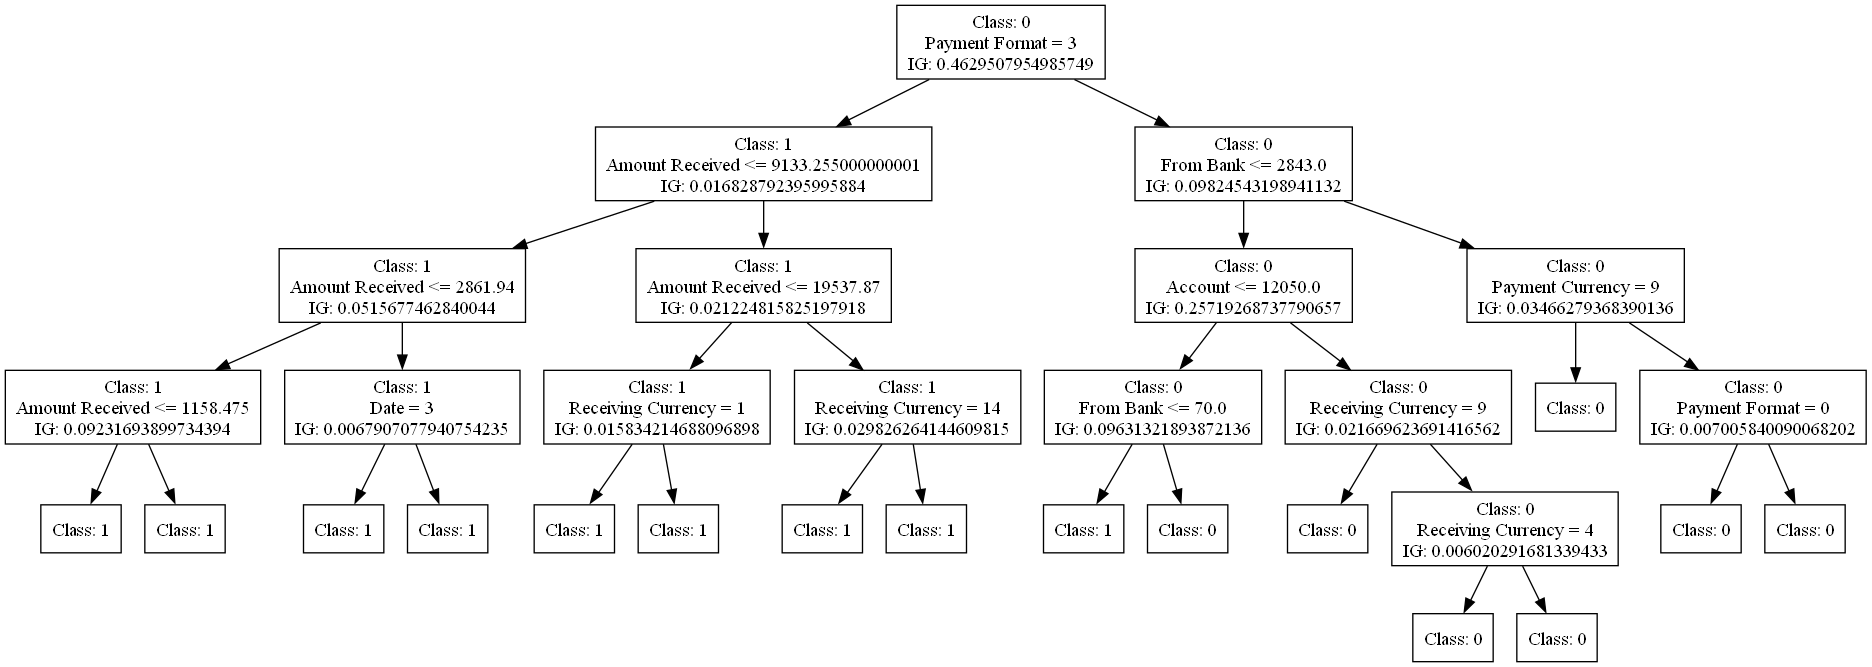
\includegraphics[width = \textwidth]{img/tree-custom-undersampling-2-1000.png}
    \caption{A representation of tree classifier generated with the custom algorithm using in the configuration with undersampling and $\phi = 20, \tau = 2, \sigma = 100$.}
    \label{fig:ex_custom_tree}
\end{figure}

\begin{table}[H]
    \centering
    {
    \footnotesize
    \begin{tabularx}{0.8 \textwidth}{|c|c|c|Y|Y|Y|Y|} 
        \hline
        & &  & \multicolumn{2}{c|}{Undersampled} & \multicolumn{2}{c|}{Oversampled} \\
        \hline
        $\phi$ & $\tau$ & $\sigma$ & $F_1$ & $Acc$ & $F_1$ & $Acc$\\
        \hline
        4 & 2 & 2 & 0.012 & 0.843 & 0.023 & 0.929\\
          &   & 100 & 0.012 & 0.843 & 0.023 & 0.929 \\
          & 4 & 2 & 0.015 & 0.885 & 0.02 & 0.917 \\
          &   & 100 & 0.015 & 0.884 & 0.02 & 0.917 \\
          & 6 & 2 & 0.015 & 0.882 & 0.021 & 0.919 \\
          &   & 100 & 0.015 & 0.882 & 0.021 & 0.919 \\
        \hline
        7 & 2 & 2 & 0.019 & 0.916 & 0.021 & 0.924 \\
          &   & 100 & 0.02 & 0.915 & 0.021 & 0.924 \\
          & 4 & 2 & 0.014 & 0.875 & 0.019 & 0.915\\
          &   & 100 & 0.014 & 0.875 & 0.019 & 0.915\\
          & 6 & 2 & 0.014 & 0.869 & 0.019 & 0.91\\
          &   & 100 & 0.014 & 0.867 & 0.02 & 0.91\\
        \hline
        10 & 2 & 2 & 0.012 & 0.911 & 0.023 & 0.932\\
          &   & 100 & 0.02 & 0.917 & 0.023 & 0.932\\
          & 4 & 2 & 0.014 & 0.878 & 0.023 & 0.932 \\
          &   & 100 & 0.014 & 0.88 & 0.021 & 0.928 \\
          & 6 & 2 & 0.016 & 0.888 & 0.021 & 0.928 \\
          &   & 100 & 0.014 & 0.876 & 0.019 & 0.92 \\
        \hline
        20 & 2 & 2 & 0.017 & 0.914 & 0.027 & 0.966 \\
          &   & 100 & 0.02 & 0.918 & 0.027 & 0.966 \\
          & 4 & 2 & 0.016 & 0.897 & 0.025 & 0.963  \\
          &   & 100 & 0.015 & 0.886 & 0.025 & 0.963  \\
          & 6 & 2 & 0.015 & 0.896 & 0.024 & 0.964 \\
          &   & 100 & 0.014 & 0.877 & 0.024 & 0.964 \\
        \hline
    \end{tabularx}
    }
    \caption{Classification performances of custom algorithm using different preprocessing techniques.}
    \label{tab:espCustom}

    % \vspace{1cm}

    % {
    % \footnotesize
    % \begin{tabularx}{0.75 \textwidth}{|c|c|Y|Y|Y|Y|} 
    %     \hline
    %      & &  \multicolumn{2}{c|}{Undersampled} & \multicolumn{2}{c|}{Oversampled} \\
    %     \hline
    %     $\phi$ & $\sigma$ & $F_1$ & $Acc$ & $F_1$ & $Acc$\\
    %     \hline
    %     4 & 2 & 0.0138 & 0.87 & 0.015 & 0.889 \\
    %       & 100 & 0.0136 & 0.869 & 0.015 & 0.889 \\
    %     8 & 2 & 0.013 & 0.862 & 0.015 & 0.883 \\
    %       & 100 & 0.013 & 0.862 & 0.015 & 0.883 \\
    %     12 & 2 & 0.013 & 0.862 & 0.015 & 0.883 \\
    %       & 100 & 0.013 & 0.862 & 0.015 & 0.883 \\
    %     \hline
    % \end{tabularx}
    % }
    % \caption{Classification performances of C4.5 by varying $\nu$ and $\sigma$ using different preprocessing techniques}
    % \label{tab:espC4.5}
    
\end{table}


\subsubsection{C4.5}

Maintaining the same analysis approach, we have evaluate a grid search over the hyperparameters $\phi \in \{4,8,12\}$ and $\sigma \in \{2, 100\}$. These hyperparameters have the same functions as in the previous algorithm.

The table \ref{tab:espC4.5} shows the classification performance of the model for these configurations.
We can observe that every pair of hyperparameters leads to very similar performances respectively in undersampling and oversampling layouts.

The execution of fitting using overfitting and prediction procedure takes about respectively 45 and 2 minutes to complete.


\begin{table}[h]
    \centering
    {
    \footnotesize
    \begin{tabularx}{0.75 \textwidth}{|c|c|Y|Y|Y|Y|} 
        \hline
         & &  \multicolumn{2}{c|}{Undersampled} & \multicolumn{2}{c|}{Oversampled} \\
        \hline
        $\phi$ & $\sigma$ & $F_1$ & $Acc$ & $F_1$ & $Acc$\\
        \hline
        4 & 2 & 0.0138 & 0.87 & 0.015 & 0.889 \\
          & 100 & 0.0136 & 0.869 & 0.015 & 0.889 \\
        8 & 2 & 0.013 & 0.862 & 0.015 & 0.883 \\
          & 100 & 0.013 & 0.862 & 0.015 & 0.883 \\
        12 & 2 & 0.013 & 0.862 & 0.015 & 0.883 \\
          & 100 & 0.013 & 0.862 & 0.015 & 0.883 \\
        \hline
    \end{tabularx}
    }
    \caption{Classification performances of C4.5 by varying $\nu$ and $\sigma$ using different preprocessing techniques}
    \label{tab:espC4.5}
\end{table} 

\subsection{Random forest}
The experiments concerning random forests are structured as follows.
A random forest is trained for each kind of previously analyzed decision tree considering the best configuration depending on preprocessing method and hyperparameters values.
Thus, these configurations are evaluated with the oversampling preprocessing method and the following hyperparameters values:
%
\begin{itemize}
    \setlength\itemsep{0cm}
    \item ID3: $\phi = 8, \ \nu = 2 $ ;
    \item Custom: $\phi = 20, \ \tau = 2, \ \sigma = 100 $ ;
    \item C4.5: $\phi = 4, \ \sigma = 100 $ .
\end{itemize}
%
We have considered as training set the 10\% of the original dataset due to execution time reasons.
Furthermore, we have used a resampling technique called bootstrap sampling \cite{IntroductionToStatisticalLearning}, which consists in randomly select $k = |T|$ observations from the dataset to obtain a new bootstrap dataset. The resampling is performed with replacement, which means that the same observation can occur more than once in the bootstrap dataset.

These settings, used to induce random forests, lead to performances reported in table \ref{tab:espRF}.
In only one case, using the custom algorithm, the generation of a random forest allows to obtain slightly better results respect to the single tree setting.

The execution of random forest in the worst case takes about 7 minutes to complete.


% All with oversampling
% ID3     F1 score: 0.000000 Accuracy: 0.998821
% Custom: F1 score: 0.002634 Accuracy: 0.996271
% C45     F1 score: 0.001210 Accuracy: 0.957748

\begin{table}[h]
    \centering
    {
    \small
    \begin{tabularx}{0.55 \textwidth}{|c|Y|Y|} 
        \hline
        Algorithm & $F_1$ & $Acc$ \\
        \hline
        ID3 & 0 & 0.998\\
        Custom & 0.003 & 0.996 \\
        C4.5 & 0.001 & 0.958\\
        \hline
    \end{tabularx}
    }
    \caption{Classification performances of random forest using different tree induction algorithms.}
    \label{tab:espRF}
\end{table}


\newpage
\addcontentsline{toc}{section}{References}
\printbibliography % [heading=none]

\end{document}
